\documentclass[tikz,border=3pt]{standalone}
\usepackage{tikz-feynman}
\begin{document}
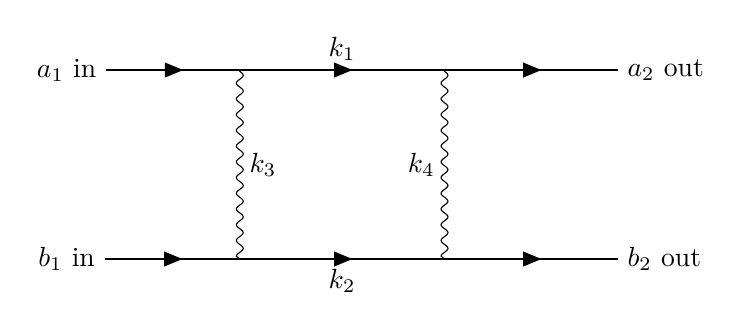
\begin{tikzpicture}
\begin{feynman}
\vertex (a1) {\(a_1\) in};
\vertex[right=2.2cm of a1] (TL);
\vertex[right=2.6cm of TL] (TR);
\vertex[right=2.2cm of TR] (a2) {\(a_2\) out};
\vertex[below=2.4cm of a1] (b1) {\(b_1\) in};
\vertex[right=2.2cm of b1] (BL);
\vertex[right=2.6cm of BL] (BR);
\vertex[right=2.2cm of BR] (b2) {\(b_2\) out};

\diagram* {
  (a1) -- [fermion] (TL) -- [fermion, edge label=\(k_1\)] (TR) -- [fermion] (a2),
  (b1) -- [fermion] (BL) -- [fermion, edge label'=\(k_2\)] (BR) -- [fermion] (b2),
  (TL) -- [photon, edge label=\(k_3\)] (BL),
  (TR) -- [photon, edge label'=\(k_4\)] (BR),
};
\end{feynman}
\end{tikzpicture}
\end{document}
